%% Produkt 1
%%%%%%%%%%%%%%%%%%%%%%%%%%%%%%
\begin{table}[!H] \centering	
	\label{fu:Fugtighedssensor}
\begin{tabular}{|p{6cm}|p{8cm}|}
	\hline
		\textbf{Løsning}				&Jord-hygrometer modul til Arduino 			\\\hline %Produktnavn
		\textbf{Producent} 			&Vides ikke 			\\\hline 
		\textbf{Tilslutning} 		&- 			\\\hline 
		\textbf{Beskrivelse} 		&En jord-fugtighedssensor, når fugtigheden er høj giver output modulet en høj værdi og omvendt ved lav fugtighed 			\\\hline 
		\textbf{Krav} 				&Indgående kendskab til PSoC creator 			\\\hline 
		\textbf{Fordele}				&Denne fugtighedssensor er klar til at blive sat i jorden, kræver ingen ekstra HW. Justerbar følsomhed via potentiometer 			\\\hline 
		\textbf{Ulemper} 			&- 			\\\hline 
		\textbf{Pris} 				&79 kr			\\\hline
		\textbf{Link} 				&\url{http://elextra.dk/main.aspx?page=article&artno=H11086	}	\\\hline  	
	
		\multicolumn{2}{|c|}
		{									%% Ændre filnavn uden endelse
		\raisebox{-0.91\height}{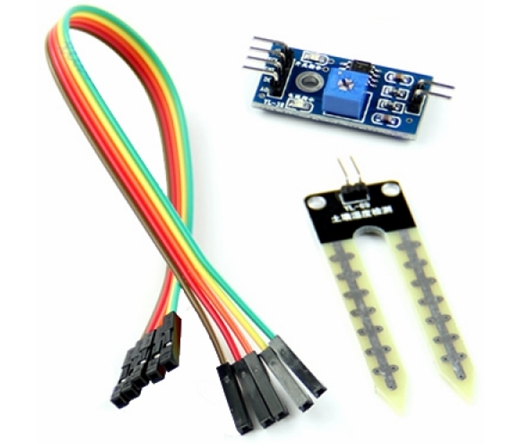
\includegraphics[height=3cm]{filer/forundersoegelse/billeder/Jord_fugt_sensor}} 
		} \\\hline	

\end{tabular}
\end{table}
%%%%%%%%%%%%%%%%%%%%%%%%%%%%%%

%% Produkt 2
%%%%%%%%%%%%%%%%%%%%%%%%%%%%%%
\begin{table}[!H] \centering	
	\label{fu:Fugtighed og temperatursensor}
\begin{tabular}{|p{6cm}|p{8cm}|}
	\hline
		\textbf{Løsning}				&SHT21P - Fugtighed og temperatur sensor IC 			\\\hline %Produktnavn
		\textbf{Producent} 			&Sensirion 			\\\hline 
		\textbf{Tilslutning} 		&Analog 			\\\hline 
		\textbf{Beskrivelse} 		&Hardware modul der giver et analog output (PWM) 			\\\hline 
		\textbf{Krav} 				&Indgående kendskab til analog signaler og PSoC creator 			\\\hline 
		\textbf{Fordele}				&Fugtighed og temperatur sensor samlet i en lille kompakt enhed. 			\\\hline 
		\textbf{Ulemper} 			&Der skal konstrueres noget HW og en ''beholder'' til sensoren så den kan tåle at komme ned i jorden 			\\\hline 
		\textbf{Pris} 				&27.55			\\\hline
		\textbf{Link} 				&\url{http://www.farnell.com/datasheets/1847262.pdf}			\\\hline	
	
	\multicolumn{2}{|c|}
	{									%% Ændre filnavn uden endelse
	\raisebox{-0.91\height}{\includegraphics[height=3cm]{filer/forundersoegelse/billeder/Fugt_temp_sensor}} 
	} \\\hline	

\end{tabular}
\end{table}
%%%%%%%%%%%%%%%%%%%%%%%%%%%%%%

%% Produkt 3
%%%%%%%%%%%%%%%%%%%%%%%%%%%%%%
\begin{table}[!H] \centering	
	\label{fu:Fugtighed og temperatursensor}
\begin{tabular}{|p{6cm}|p{8cm}|}
	\hline
		\textbf{Løsning}				&SHT71P - Fugtighed og temperatur sensor IC 			\\\hline %Produktnavn
		\textbf{Producent} 			&Sensirion 			\\\hline 
		\textbf{Tilslutning} 		&I2C Variation 			\\\hline 
		\textbf{Beskrivelse} 		&Hardware modul der kommunikeres med via en I2C variation 			\\\hline 
		\textbf{Krav} 				&Indgående kendskab til I2C kommunikation og PSoC creator 			\\\hline 
		\textbf{Fordele}				&Fugtighed og temperatur sensor samlet i en lille kompakt enhed. 			\\\hline 
		\textbf{Ulemper} 			&Der skal konstrueres noget HW og en "beholder" til sensoren så den kan tåle at komme ned i jorden 			\\\hline 
		\textbf{Pris} 				&Hentes i værkstedet			\\\hline
		\textbf{Link} 				&\url{http://www.sensirion.com/fileadmin/user_upload/customers/sensirion/Dokumente/Humidity/Sensirion_Humidity_SHT7x_Datasheet_V5.pdf}			\\\hline	
	
	\multicolumn{2}{|c|}
	{									%% Ændre filnavn uden endelse
	\raisebox{-0.91\height}{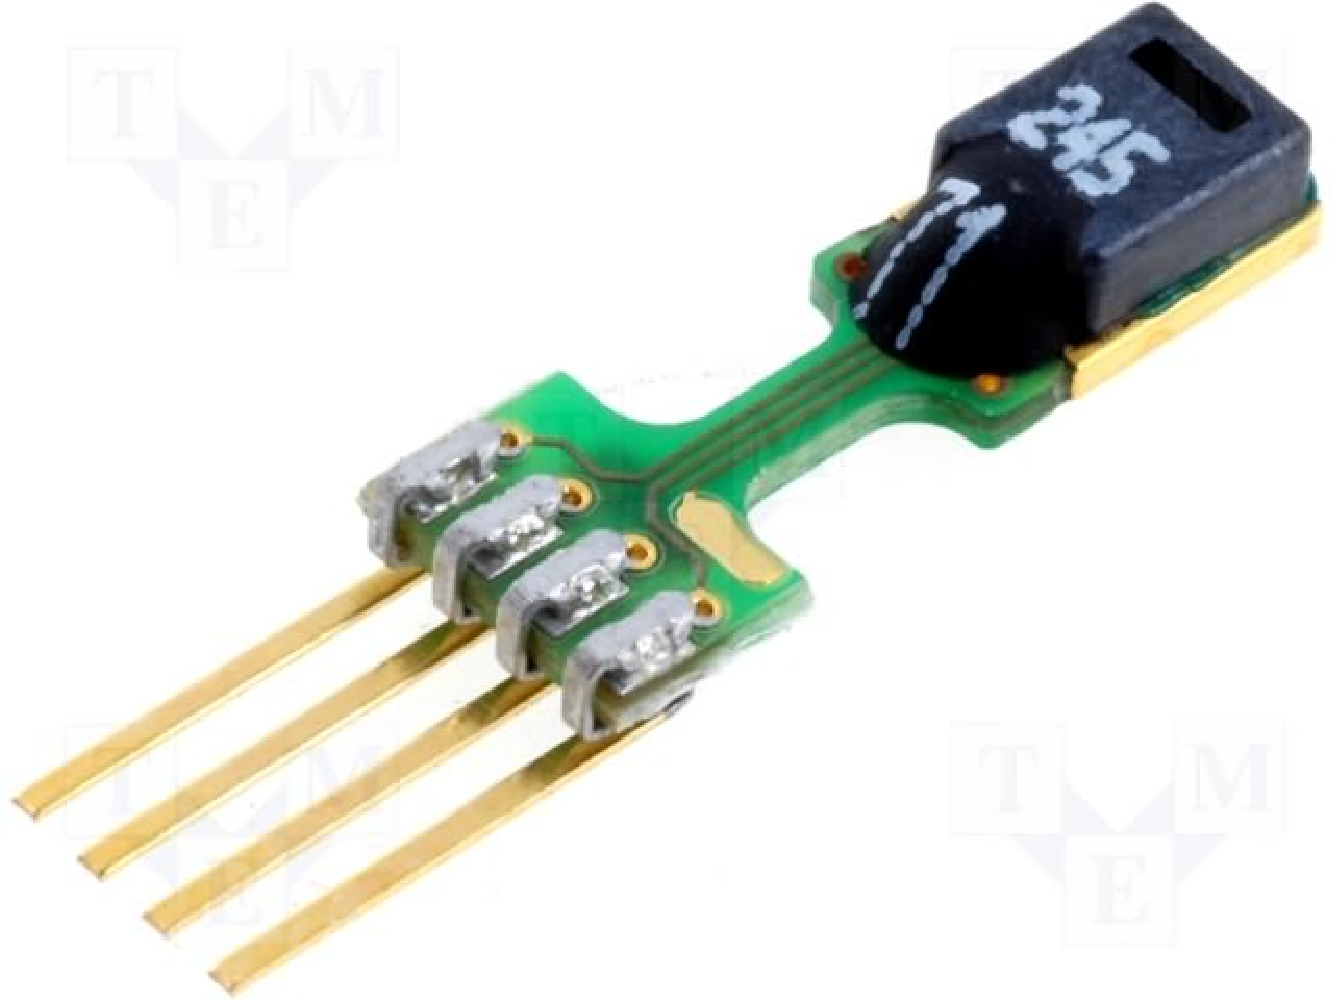
\includegraphics[height=3cm]{filer/forundersoegelse/billeder/Sensirion-SHT71-image.pdf}} 
	} \\\hline	

\end{tabular}
\end{table}
%%%%%%%%%%%%%%%%%%%%%%%%%%%%%%